\section{Requisitos Funcionales}

Los requisitos funcionales describen las funcionalidades esenciales que debe cumplir la aplicación para satisfacer las necesidades del usuario. En el caso de esta aplicación, todos los requisitos funcionales están orientados al cumplimiento del objetivo principal: permitir a los usuarios acceder al análisis de sus datos musicales cuando lo deseen. Estas funcionalidades están organizadas en diferentes categorías según su ámbito.

\subsection{Autenticación y Sesión}
\begin{itemize}
    \item El usuario debe poder iniciar sesión utilizando su cuenta de \textit{Spotify} mediante OAuth 2.0.
    \item El usuario debe poder cerrar sesión desde cualquier página.
    \item El cierre de sesión debe eliminar cualquier dato asociado al usuario.
    \item La aplicación debe obtener y gestionar adecuadamente e token de acceso para interactuar con la API de \textit{Spotify}.
    \item La sesión del usuario debe permanecer activa mientras este interactúe con la aplicación web. En caso de que el tiempo de validez del token expire, el sistema debe renovar el token de forma transparente para el usuario.
\end{itemize}

\subsection{Navegación}
\begin{itemize}
    \item La aplicación debe tener una barra de navegación con acceso a las secciones:
          \begin{itemize}
              \item \textbf{Home:} Vista general de las estadísticas generales.
              \item \textbf{Stats:} Estadísticas más avanzadas y originales.
              \item \textbf{Panel de Usuario:} Panel desplegable con la opción de cerrar sesión. % y botón de ajustes
          \end{itemize}
\end{itemize}

\subsection{Estadísiticas Generales (Home)}
\begin{itemize}
    \item El usuario debe ver una página inicial con estadísticas generales relacionadas con su cuenta, siendo las siguientes:
          \begin{itemize}
              \item \textbf{Top Tracks:} Muestra los top 5 canciones del usuario.
              \item \textbf{Top Artists:} Muestra los top 5 artistas del usuario.
              \item \textbf{Top Genres:} Muestra los top 5 géneros del usuario,
              \item \textbf{Recently Played:} Muestra una lista reducida de las últimas 10 canciones escuchadas, en orden cronológico. Si el usuario quiere, podrá ver la lista completa de las 50 canciones pulsando un botón.
          \end{itemize}
    \item El usuario podrá cambiar el periodo de tiempo en el que se basan los datos de los tres tops mediante un menú desplegable.
\end{itemize}

\subsection{Estadísticas Avanzadas (Stats)}

En esta página, el usuario podrá explorar una gama de seis estadísticas más avanzadas. Cada estadística ofrece funcionalidades específicas, descritas a continuación:

\subsubsection*{Hall Of Fame}

\begin{itemize}
    \item La estadística mostrará las \textbf{top 16 canciones} del usuario en formato de cuadrícula (4x4), utilizando las portadas de los álbumes de cada canción como elemento visual.
    \item Al pasar el ratón por encima de cada una de las portadas, se mostrará el nombre de la canción y el artista.
    \item El usuario, mediante un botón, podrá crear una playlist de manera automática en su cuenta:
          \begin{itemize}
              \item Se generará una nueva playlist.
              \item Se añadirán las canciones del top 16.
              \item Se actualizará la imagen de la playlist con la representación visual de la cuadrícula de portadas generada para esta estadística.
          \end{itemize}
\end{itemize}

\subsubsection*{Huella Del Día}

% TODO: Un poco justillo la interactividad en esta estadística.
\begin{itemize}
    \item El usuario verá un gráfico de líneas, donde el eje horizontal representa las horas del día y el eje vertical los minutos de música escuchados (correspondientes a 1 hora).
    \item Al pasar el ratón por encima de un nodo de la gráfica, se mostrará la cantidad exacta de minutos escuchados en esa hora.
    \item Se indica la hora del día con más minutos de escucha.
\end{itemize}

\subsubsection*{Estaciones Musicales}

\begin{itemize}
    \item Se mostrará un gráfico en forma de anillo dividido en cuatro segmentos, cada uno representando una estación del año: invierno, primavera, verano y otoño.
    \item Al pasar el ratón por encima de un segmento del gráfico, se abrirá un panel que mostrará, basado en la actividad del usuario, el artista y el género musical destacados durante ese periodo.
    \item La información en el panel se actualiza dinámicamente mientras el usuario pasa el ratón por las distintas secciones del gráfico.
\end{itemize}

\subsubsection*{Tus Décadas}

\begin{itemize}
    \item Se presentará un histograma que muestra el número de álbumes correspondientes a cada año, agrupados por décadas. La cantidad de álbumes se muestra de manera visual, mediante imágenes de portadas apiladas en columnas. Los álbumes están asociados a las canciones favoritas del usuario, mostrando una única repetición de cada álbum, independientemente de la cantidad de canciones guardadas de ese álbum.
    \item El gráfico es explorable, permitiendo al usuario desplazarse horizontal y verticalmente.
    \item El usuario podrá hacer \textit{zoom in} y \textit{zoom out} para ajustar el nivel de detalle, permitiéndole observar las portadas de los álbumes con mayor claridad.
\end{itemize}

\subsubsection*{La Bitácora}

El usuario podrá explorar detalladamente el historial completo de sus canciones guardadas en favoritos, organizadas por fechas. Se estructura de la siguiente manera:
\begin{itemize}
    \item Se mostrará la visualización principal; un gráfico de barras con el número total de canciones guardadas, agrupadas por años, desde la creación de la cuenta hasta la fecha actual.
    \item Al hacer clic en una barra que represente un año, se profundizará en el gráfico para mostrar la distribución de canciones guardadas por meses dentro de ese año.
    \item De forma similar, al hacer clic en una barra que represente un mes, se desglosará la información para mostrar las canciones guardadas por días dentro de ese mes específico.
    \item El usuario podrá navegar libremente entre los niveles (años, meses y días), pudiendo retroceder hacia niveles superiores en cualquier momento.
    \item Al pasar el ratón por encima de cualquier barra, se mostrará el número de canciones guardadas para ese período.
    \item En el nivel de días, al pasar el ratón sobre una barra, se mostrarán además los nombres y artistas de las canciones guardadas en esa fecha específica.
\end{itemize}


\subsubsection*{Índice de Resonancia}

Se presentará al usuario, de forma visual, dos métricas relacionadas con sus preferencias musicales: la popularidad media de sus canciones guardadas en favoritos y la popularidad media de las últimas 50 canciones escuchadas. Estas métricas se implementarán a través de las siguientes funcionalidades:
\begin{itemize}
    \item Cada valor estará asociado a una onda sinusoidal animada, cuya frecuencia se ajustará proporcionalmente al valor numérico correspondiente.
    \item El usuario podrá pulsar un botón que generará una nueva onda. Esta nueva onda se calcula mediante la suma matemática de las frecuencias de las dos ondas originales, mostrando la interferencia entre las dos. Además, junto a esta nueva onda, se mostrará la diferencia numérica entre los dos valores originales.
    \item El usuario podrá pasar el ratón sobre la tarjeta de cualquiera de los valores para resaltar visualmente la onda correspondiente, facilitando la identidicación.
    \item Los cálculos y la generación de datos necesarios para esta estadística se realizarán principalmente en el servidor.
\end{itemize}

\section{Requisitos No Funcionales}

Los requisitos no funcionales de la aplicación son fundamentales para garantizar no solo su funcionalidad, sino también su rendimiento, seguridad, escalabilidad y usabilidad. A continuación, se detallan los aspectos clave que la aplicación debe cumplir para asegurar una experiencia de usuario satisfactoria y el cumplimiento de los estándares de calidad.

\subsection*{Seguridad}

Es esencial garantizar la protección de los datos del usuario y las comunicaciones entre el frontend y el backend. Para ello, todas las conexiones deben utilizar \textbf{HTTPS}, y los tokens de acceso deben almacenarse de forma segura para prevenir ataques comunes como \textit{Cross-Site Scripting} (XSS) y \textit{Man-in-the-Middle} (MITM). Además, es necesario implementar medidas de seguridad en procesos críticos, como la autenticación de usuarios, incluyendo protección frente a ataques de tipo \textit{Cross-Site Request Forgery} (CSRF).

\subsection*{Testabilidad}

Para garantizar la calidad del sistema, se deben implementar pruebas automatizadas que cubran las funcionalidades clave de la aplicación, priorizando las partes críticas del backend y las interacciones más relevantes del frontend. Esto incluirá pruebas unitarias y de integración. La cobertura mínima objetivo será del \textbf{60\% del código}, con un enfoque en las secciones esenciales. Las pruebas se ejecutarán regularmente mediante integración continua (CI) utilizando GitHub Actions.

\subsection*{Usabilidad}

La aplicación debe ser intuitiva y fácil de usar para el público general. Todas las estadísticas y funcionalidades deben presentarse de manera clara. Este requisito se evaluará mediante pruebas de usabilidad con al menos \textbf{5 usuarios representativos}, asegurando que puedan completar tareas concretas sin dificultad ni confusión.


\section{Casos de Uso}

En esta sección se describen los principales casos de uso de la aplicación, relacionados con los requisitos funcionales mencionados. Cada caso de uso se enfoca en un objetivo específico que un usuario puede alcanzar utilizando las funcionalidades del sistema.

\subsection{Actores}

En este sistema, interactúan tres actores diferentes con la aplicación: el usuario anónimo, el usuario autenticado y la API de \textit{Spotify}. A continuación, se describen los roles de cada uno:

\begin{itemize}
    \item \textbf{Usuario Anónimo:} Este actor representa a los usuarios que no han iniciado sesión en la aplicación. Su única interacción con el sistema es el de inicio de sesión.
    \item \textbf{Usuario Autenticado:} Este actor es el usuario que ha iniciado sesión correctamente en la aplicación. Tiene acceso a todas las funcionalidades. Es considerado como el actor principal.
    \item \textbf{Web API de Spotify:} Este actor es el servicio de \textit{Spotify} que proporciona un sistema de autenticación y los datos necesarios para generar las estadísticas. Interactúa principalmente con el backend de la aplicación.
\end{itemize}


\subsection{Modelo de Casos de Uso}

En el modelo presentado en la figura \ref{fig:modelo_casos_uso}, se destacan las funcionalidades principales de la aplicación y su relación con los actores: \textbf{Usuario Anónimo} y \textbf{Usuario Autenticado}, que interactúan directamente con el sistema, y la \textbf{API de Spotify}, que actúa como proveedor de datos.

\begin{figure}[H]
    \centering
    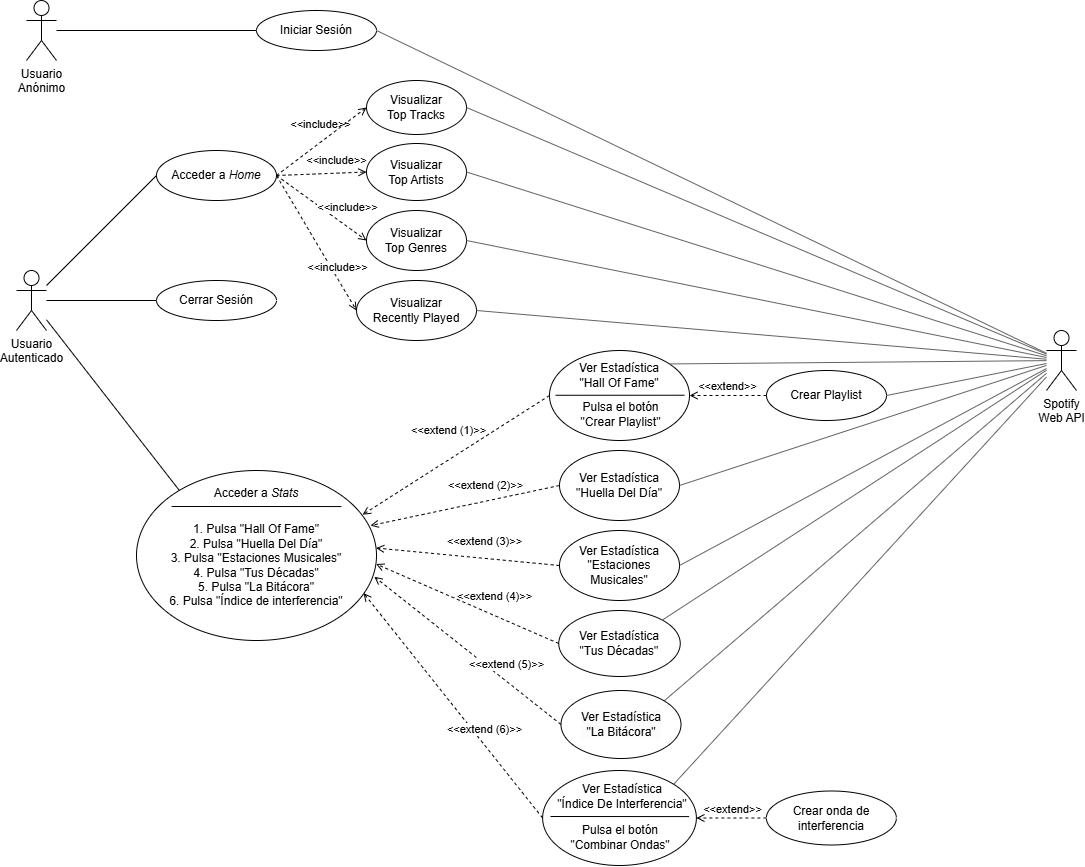
\includegraphics[width=\textwidth]{figures/modelo_casos_uso.png}
    \caption{Modelo de casos de uso del sistema.}
    \label{fig:modelo_casos_uso}
\end{figure}

% TODO: Decir dónde estarán los diagramas de secuencia.

\subsubsection*{Iniciar Sesión}

Permite al usuario anónimo iniciar sesión en la aplicación utilizando sus credenciales de \textit{Spotify} a través del sistema de autenticación OAuth 2.0.

\begin{itemize}
    \item Flujo principal (Inicio de Sesión):
          \begin{enumerate}
              \item El usuario anónimo selecciona la opción de ``Iniciar Sesión'' en la pantalla principal.
              \item El sistema redirige al usuario a la página de inicio de sesión de \textit{Spotify}.
              \item El usuario introduce sus credenciales de \textit{Spotify} en el formulario proporcionado por \textit{Spotify}.
              \item \textit{Spotify} verifica las credenciales y, si son correctas, muestra la pantalla de solicitud de autorización.
              \item El usuario autoriza a la aplicación a acceder a sus datos de \textit{Spotify} indicados.
              \item \textit{Spotify} genera un token de acceso y redirige al usuario de vuelta a la aplicación.
              \item El sistema recibe el token de acceso y lo almacena de forma segura.
              \item El sistema redirige al usuario autenticado a la pantalla principal de la aplicación (\textit{Home}).
          \end{enumerate}
    \item Flujo alternativo (Error de Autenticación):
          \begin{enumerate}
              \item El usuario introduce credenciales incorrectas en la página de inicio de sesión de \textit{Spotify}.
              \item \textit{Spotify} rechaza las credenciales y muestra un mensaje de error al usuario.
              \item El sistema redirige al usuario de vuelta a la pantalla principal, donde podrá volver a intentar iniciar sesión.
          \end{enumerate}
    \item Flujo alternativo (Denegación de Autorización):
          \begin{enumerate}
              \item \textit{Spotify} verifica las credenciales del usuario y muestra la pantalla de solicitud de autorización.
              \item El usuario decide no conceder la autorización y selecciona la opción de ``Cancelar''.
              \item \textit{Spotify} informa al sistema de que la autorización ha sido rechazada.
              \item El sistema redirige al usuario de vuelta a la pantalla principal.
          \end{enumerate}
\end{itemize}

\subsubsection*{Acceder a Home}

Permite al usuario autenticado visualizar la pantalla principal de la aplicación, donde se muestran las estadísticas básicas de \textit{Top Tracks}, \textit{Top Artists}, \textit{Top Genres} y \textit{Recently Played}.

\begin{itemize}
    \item Flujo principal (Visualización de Home):
          \begin{enumerate}
              \item El usuario autenticado accede a la aplicación tras iniciar sesión correctamente.
              \item El sistema solicita los datos relevantes de la API de \textit{Spotify} para generar las estadísticas.
              \item La API de \textit{Spotify} responde con los datos necesarios para cada estadística.
              \item El sistema procesa y organiza los datos para presentarlos en el frontend.
              \item El sistema muestra al usuario las siguientes secciones en la pantalla principal:
                    \begin{itemize}
                        \item \textit{Top Tracks}: Canciones más escuchadas por el usuario.
                        \item \textit{Top Artists}: Artistas más escuchados.
                        \item \textit{Top Genres}: Géneros favoritos.
                        \item \textit{Recently Played}: Lista de reproducción reciente.
                    \end{itemize}
              \item El usuario puede cambiar el periodo de tiempo de las estadísticas de los tres \textit{Tops} seleccionando entre los últimos 30 días, 6 meses o 1 año.
              \item El usuario puede expandir la lista de \textit{Recently Played} para ver hasta 50 canciones en lugar de las 10 iniciales, pulsando un botón de "Ver más".
              \item El usuario puede contraer nuevamente la lista de \textit{Recently Played} para reducirla a 10 canciones, pulsando un botón de "Ver menos".
          \end{enumerate}
    \item Flujo alternativo (Error al obtener datos de la API):
          \begin{enumerate}
              \item El sistema solicita datos a la API de \textit{Spotify}, pero ocurre un error en la comunicación.
              \item El sistema muestra un mensaje de error al usuario, indicando que no se pudieron cargar algunas estadísticas.
              \item El usuario puede intentar recargar la página o esperar a que el sistema reintente la solicitud.
          \end{enumerate}
\end{itemize}

\subsubsection*{Cerrar Sesión}

Permite al usuario autenticado cerrar su sesión en la aplicación, eliminando cualquier dato relacionado con su sesión activa.

\begin{itemize}
    \item Flujo principal (Cerrar Sesión):
          \begin{enumerate}
              \item El usuario autenticado selecciona la opción de ``Cerrar Sesión'' en la interfaz de la aplicación.
              \item El sistema elimina todas las cookies relacionadas con la sesión, incluido el \textit{access\_token} del usuario.
              \item El sistema borra cualquier dato del usuario almacenado temporalmente en caché.
              \item El sistema redirige al usuario a la página de inicio de sesión.
          \end{enumerate}
\end{itemize}

\subsubsection*{Acceder a Stats}

Permite al usuario autenticado acceder a la sección de estadísticas avanzadas de la aplicación, donde puede interactuar con diferentes visualizaciones de sus datos musicales.

\begin{itemize}
    \item Flujo principal (Acceso a Stats):
          \begin{enumerate}
              \item El usuario autenticado selecciona la opción de ``Stats'' en la barra de navegación.
              \item El sistema muestra una pantalla con las opciones de estadísticas disponibles:
                    \begin{itemize}
                        \item \textbf{Hall of Fame.}
                        \item \textbf{Huella del Día.}
                        \item \textbf{Estaciones Musicales.}
                        \item \textbf{Tus Décadas.}
                        \item \textbf{La Bitácora.}
                        \item \textbf{Índice de Interferencia.}
                    \end{itemize}
              \item El usuario selecciona una estadística específica para interactuar con ella.
              \item El sistema carga la visualización correspondiente.
          \end{enumerate}
\end{itemize}

Para todas las siguientes estadísticas avanzadas, se sigue un flujo alternativo cuando ocurre algún error en la carga. Para evitar repetir la misma descripción, a continuación se mencionará el flujo alternativo. En cada estadística, solo se describirá el flujo principal.

\begin{itemize}
    \item Flujo alternativo (Error en la carga de datos de una estadística avanzada):
          \begin{enumerate}
              \item El sistema solicita a la API de \textit{Spotify} los datos necesarios para generar la estadística.
              \item La API responde con un error, ya sea por una conexión fallida, un token de acceso inválido o una respuesta incompleta.
              \item El sistema muestra un mensaje de error en la pantalla, indicando que no se pudo cargar la estadística.
          \end{enumerate}
\end{itemize}

\subsubsection*{Ver Estadística: Hall of Fame}

Permite al usuario visualizar las 16 canciones más destacadas según su actividad, representadas en forma de cuadrícula con las portadas de los álbumes correspondientes.

\begin{itemize}
    \item Flujo principal (Visualización de Hall of Fame):
          \begin{enumerate}
              \item El usuario selecciona la opción ``Hall of Fame'' en la pantalla de \textit{Stats}.
              \item El sistema solicita a la API de \textit{Spotify} las 16 canciones más destacadas del usuario.
              \item La API responde con los datos necesarios, incluyendo nombres, artistas y portadas de los álbumes.
              \item El sistema genera una cuadrícula con las portadas de los álbumes correspondientes.
              \item El usuario puede pasar el ratón sobre una portada para visualizar el nombre de la canción y el artista.
              \item Si el usuario pulsar el botón ``Crear Playlist'', se envía la portada generada y los datos de las canciones a la API de \textit{Spotify} para crear una nueva playlist.
          \end{enumerate}
\end{itemize}

\subsubsection*{Ver Estadística: Huella del Día}

Permite al usuario visualizar un gráfico de línea que representa los minutos escuchados por cada hora del día, mostrando las horas de mayor actividad musical.

\begin{itemize}
    \item Flujo principal (Visualización de Huella del Día):
          \begin{enumerate}
              \item El usuario selecciona la opción ``Huella del Día'' en la pantalla de \textit{Stats}.
              \item El sistema solicita a la API de \textit{Spotify} los datos de escucha del usuario necesarios para calcular los minutos por hora.
              \item La API responde con los datos correspondientes.
              \item El sistema genera el gráfico de línea.
              \item El usuario puede pasar el ratón sobre los puntos de la línea para ver los minutos escuchados en una hora específica.
              \item El sistema destaca visualmente la hora con más minutos escuchados.
          \end{enumerate}
\end{itemize}

\subsubsection*{Ver Estadística: Estaciones Musicales}

Permite al usuario visualizar, de forma gráfica, el artista y género más representativo de cada estación del año según su actividad musical.

\begin{itemize}
    \item Flujo principal (Visualización de Estaciones Musicales):
          \begin{enumerate}
              \item El usuario selecciona la opción ``Estaciones Musicales'' en la pantalla de \textit{Stats}.
              \item El sistema solicita a la API de \textit{Spotify} los datos necesarios para calcular el artista y género destacados de cada estación.
              \item La API responde con los datos correspondientes.
              \item El sistema calcula los datos y los agrupa por estaciones.
              \item El sistema genera un gráfico de tipo anillo dividido en cuatro segmentos, representando cada estación del año.
              \item El usuario puede pasar el ratón sobre uno de los segmentos del gráfico para que el sistema muestre, en un panel adicional, el artista y género destacados de la estación seleccionada.
              \item El sistema actualiza el panel dinámicamente según el segmento que el usuario seleccione con el ratón.
          \end{enumerate}
\end{itemize}

\subsubsection*{Ver Estadística: Tus Décadas}

Permite al usuario visualizar en formato de histograma los álbumes de sus canciones favoritas organizados por décadas, destacando las épocas más representativas de su actividad musical.

\begin{itemize}
    \item Flujo principal (Visualización de Tus Décadas):
          \begin{enumerate}
              \item El usuario selecciona la opción ``Tus Décadas'' en la pantalla de \textit{Stats}.
              \item El sistema solicita a la API de \textit{Spotify} los datos de las canciones guardadas por el usuario en su biblioteca.
              \item La API responde con los datos, incluyendo las fechas de lanzamiento de los álbumes asociados a las canciones.
              \item El sistema organiza los datos por décadas y genera el histograma correspondiente.
              \item El usuario puede desplazarse sobre el gráfico arrastrando con el ratón y explorar con mayor detalle las portadas, ampliando o reduciendo el aumento, mediante la rueda de desplazamiento.
          \end{enumerate}
\end{itemize}

\subsubsection*{Ver Estadística: La Bitácora}

Permite al usuario explorar el historial completo de sus canciones guardadas en favoritos, organizadas cronológicamente.

\begin{itemize}
    \item Flujo principal (Visualización de La Bitácora):
          \begin{enumerate}
              \item El usuario selecciona la opción ``La Bitácora'' en la pantalla de \textit{Stats}.
              \item El sistema solicita a la API de \textit{Spotify} los datos de las canciones guardadas en favoritos, incluyendo la fecha en que fueron añadidas.
              \item La API responde con los datos correspondientes.
              \item El sistema genera un gráfico de barras que muestra, inicialmente, el número de canciones guardadas por año.
              \item El usuario puede interactuar con el gráfico para explorar diferentes niveles de detalle:
                    \begin{itemize}
                        \item Al hacer clic en una barra que representa un año, el sistema actualiza el gráfico para mostrar los meses dentro de ese año.
                        \item Al hacer clic en una barra que representa un mes, el sistema desglosa la información para mostrar los días dentro de ese mes.
                    \end{itemize}
              \item Al pasar el ratón sobre cualquier barra, el sistema muestra un tooltip con el número de canciones guardadas en ese periodo.
              \item El usuario puede navegar libremente entre los niveles (años, meses y días) y retroceder en cualquier momento para cambiar de periodo.
          \end{enumerate}
\end{itemize}

\subsubsection*{Ver Estadística: Índice de Interferencia}

Permite al usuario comparar el cambio en sus gustos sobre la popularidad de las canciones que escucha.

\begin{itemize}
    \item Flujo principal (Visualización de Índice de Interferencia):
          \begin{enumerate}
              \item El usuario selecciona la opción ``Índice de Interferencia'' en la pantalla de Stats.
              \item El sistema solicita a la API de \textit{Spotify} los datos necesarios.
              \item La API responde con los datos correspondientes.
              \item El sistema hace el cálculo de las dos popularidades medias y los presenta visualmente en forma de ondas sinusoidales animadas.
              \item Si el usuario pulsa un botón de ``Combinar Ondas'', el sistema genera una nueva onda, resultado de la suma matemática de las frecuencias de las dos ondas originales (interferencia).
              \item El sistema muestra esta nueva onda junto a la diferencia numérica entre las dos popularidades.
          \end{enumerate}
\end{itemize}
